% !TeX program = xelatex
\documentclass[UTF8,fontset=fandol,11pt]{ctexart}
\usepackage[a4paper,margin=2.15cm]{geometry}
\usepackage{amsmath,amssymb,bm,booktabs,multirow,graphicx,float,subcaption}
\usepackage[numbers,sort&compress]{natbib}
\usepackage[colorlinks=true,citecolor=blue,urlcolor=blue,linkcolor=blue]{hyperref}
\newcommand{\ModelParams}{276,801}
\newcommand{\UniqueMean}{0.479}
\newcommand{\UniqueQ}{0.507}
\newcommand{\UniqueMax}{0.521}
\newcommand{\WorstAUC}{0.876}

\newcommand{\method}{HKReal3DMark}
\title{\method：面向香港实景三维网格版权认证的\\轻量鲁棒零水印方法}
\author{作者信息待定\quad 指导教师信息待定}
\date{}
\begin{document}\maketitle
\begin{abstract}
实景三维城市模型由倾斜摄影测量重建而成，具有数据规模大、生产成本高、易于无损复制和跨格式传播等特点。传统嵌入式网格水印需要修改顶点、连接关系或纹理，可能影响测绘成果精度；现有零水印多依赖人工径向统计，在强裁剪和相似城市瓦片之间容易出现鲁棒性与唯一性冲突。本文提出\method，一种直接面向Cesium/B3DM实景三维网格的轻量学习式零水印框架。方法从三角网格确定性采样点集，经稳健中心、尺度和主轴规范化后，以共享点编码、注意力汇聚及径向分位数融合提取内容表示；采用原始--攻击多视图对比学习、软比特最差视图一致性和异源分离约束学习攻击不变量；登记阶段冻结编码器，仅优化密钥化1024-bit投影。本文基于香港地政总署全港三维视觉化地图建立严格地域隔离的120模型数据集，考察旋转、缩放、噪声、量化、删点、简化、空间裁剪、离群点及连续复合攻击。固定随机种子2026的RTX~4090实验表明，测试登记库异源NC均值、q95和最大值分别为\UniqueMean、\UniqueQ 和\UniqueMax；旋转、尺度、噪声和量化的全部强度AUC均为1.000，80\%随机删点和连续复合攻击的AUC分别为0.957和1.000，所有设置中的最差AUC为\WorstAUC。结果说明，可靠零水印必须同时评价同源NC、异源唯一性和认证可分性，而不能仅追求攻击后高NC。
\end{abstract}
\noindent\textbf{关键词：}实景三维；零水印；三维网格；对比学习；Cesium；版权认证

\section{引言}
大范围实景三维数据已成为数字孪生城市、规划分析和空间治理的重要底座。香港地政总署公开的三维视觉化地图覆盖建筑、基础设施、植被、水体和地形等对象，并提供个体模型、分块模型和无纹理模型等产品\cite{Open3Dhk}。其中分块模型由倾斜航空影像重建为带纹理三角网格，并通过Cesium 3D Tiles/B3DM组织多级细节。它属于广义城市三维空间数据，但与CityGML不同：B3DM主要承载网格几何、纹理和空间层级，不提供Building、RoofSurface等显式城市对象语义。本文因此将研究对象严格称为“实景三维网格”，而不将其误写为CityGML语义CIM。

实景三维成果可被完整复制、局部裁剪、重新采样、降面或格式转换。三维网格嵌入式水印通过改变顶点或变换系数携带比特，需在不可感知性、容量与鲁棒性之间折衷\cite{WangSurvey2008,WangDeepMesh2022,ZhuDeep3DMark2024}。测绘数据对几何精度和成果可追溯性要求较高，任何坐标修改都可能引发工程风险。零水印从载体提取内容指纹，在外部登记内容指纹与所有者二值水印的组合证据，不修改原始模型，因而更契合该场景。

现有三维零水印多使用顶点范数直方图、多特征稳定顶点或球坐标统计\cite{Jiang2018,Wang2019,Lee2021}。人工特征具有明确的刚体不变性，却未必能区分统计分布相近的城市瓦片。如果所有模型都映射为相似码字，攻击前后NC会很高，但系统无法判断版权归属。学习方法可以利用多攻击视图学习稳定且有区分性的表示，对比学习已在视觉表示中证明其有效性\cite{Chen2020}，点云网络则提供了处理无序点集的可行范式\cite{PointNet}。

本文贡献如下：
\begin{enumerate}
\item 建立香港实景三维B3DM端到端零水印流程，包括网格解析、确定性点采样、稳健规范化、地域隔离划分、攻击、登记和认证，全流程不修改源模型。
\item 提出轻量局部--全局融合编码器，以共享点特征、三种集合池化和径向分位数表征网格，并通过多视图对比、最差视图软比特约束及身份分离学习攻击不变量。
\item 设计仅投影个性化登记。编码器保持冻结，由干净登记模型在线生成多尺度视图，只优化密钥投影，使鲁棒性增强不以指纹坍缩为代价。
\item 在15个一级区域构成的地域隔离协议上评估九类攻击强度曲线，与三类同数据人工特征基线比较，同时报告平均NC、尾部NC、异源q95、AUC和EER。
\end{enumerate}

\section{相关工作}
\subsection{三维网格水印与零水印}
三维网格水印可分为嵌入式和零水印两类。嵌入式方法将信息写入顶点坐标、谱系数或局部几何，深度模型进一步联合学习嵌入和提取\cite{WangDeepMesh2022,ZhuDeep3DMark2024}；优点是水印随载体传播，缺点是必须改变数据。零水印不修改载体，而是提取稳定特征后与所有者水印异或或加密登记。Jiang和Kim针对CityGML使用归一化顶点范数直方图生成零水印\cite{Jiang2018}；Wang等融合稳定顶点、形状直径和统计矩\cite{Wang2019}；Lee等依据球坐标分组和偏度构造稳健比特\cite{Lee2021}。这些工作为刚体不变特征提供基础，但其输入和攻击协议与摄影测量分块网格并不完全相同。

\subsection{学习式三维表示与对比学习}
PointNet以共享多层感知机和对称函数直接处理无序点集\cite{PointNet}，PointNet++通过局部层级采样增强细节表达\cite{PointNetPP}，动态图网络进一步建模邻域关系\cite{DGCNN}。本文不追求大型分类骨干，而是使用不足30万参数的共享点编码器，并保留人工径向分位数分支。与嵌入式深度水印不同，网络只输出内容表示，二值水印证据登记在模型外部。

SimCLR通过同一样本的增强视图构造正对、其他样本构造负对\cite{Chen2020}。零水印比普通检索更强调攻击视图一致性：平均稳定并不足够，最强视图的比特翻转可能使认证失败。因此本文在多正样本对比之外，对各攻击视图的软比特误差加入最大项，并惩罚不同模型之间的正相关。

\section{方法}
\subsection{问题定义与威胁模型}
设实景三维网格为$M=(V,F)$，$V\in\mathbb R^{n\times3}$为顶点，$F$为三角面。内容编码器$E_\theta$和密钥投影$P_\kappa$产生$B$位指纹
\begin{equation}\bm b(M)=\mathbb I[P_\kappa E_\theta(M)\ge0],\qquad B=1024.\end{equation}
对攻击$T$，同源分数$s^+=\operatorname{NC}(\bm b(M),\bm b(T(M)))$；不同模型$M_i,M_j$的异源分数$s^-=\operatorname{NC}(\bm b(M_i),\bm b(M_j))$。本文使用归一化Hamming相似度
\begin{equation}\operatorname{NC}(\bm b_i,\bm b_j)=\frac1B\sum_{k=1}^{B}\mathbb I[b_{ik}=b_{jk}].\end{equation}
可靠认证要求$s^+$整体高于$s^-$，而不仅是$s^+$绝对值较高。攻击者可进行常见几何编辑，但不知道私有投影和登记码本；密钥泄露与白盒对抗攻击不在本文范围。

\subsection{B3DM解析与稳健规范化}
B3DM容器由头部、feature/batch table和内嵌GLB组成。解析全部scene node变换后，将几何体顶点变换到统一坐标系。按照源文件相对路径的SHA-256摘要生成采样种子，从每个瓦片确定性采样$N=1024$个点。

令点集为$X$。首先减去逐维中位数$\bm m$，再以中心距离的截尾95\%分位数归一化尺度：
\begin{equation}X_c=X-\bm m,\quad s=Q_{0.95}(\{\|\bm x\|_2:\bm x\in X_c^{80\%}\}),\quad \widehat X=X_c/(s+\epsilon).\end{equation}
$X_c^{80\%}$表示删除半径最大20\%点后的子集。由其协方差特征向量构建PCA主轴，并利用三阶中心矩确定轴方向，最终坐标截断至$[-3,3]$。干净与攻击分支执行完全相同的规范化，避免预处理差异被误计为攻击误差。

\subsection{轻量局部--全局融合编码器}
对每个点构造七维输入$\bm f_i=[x_i,y_i,z_i,|x_i|,|y_i|,|z_i|,\|\bm x_i\|_2]$。共享MLP将其映射为128维局部表示$\bm h_i$。通过均值、最大和注意力三种函数汇聚：
\begin{equation}\bm g=[\operatorname{mean}_i\bm h_i;\operatorname{max}_i\bm h_i;\sum_i\alpha_i\bm h_i;\bm q_r],\end{equation}
其中$\alpha_i=\operatorname{softmax}(\bm w^T\bm h_i)$，$\bm q_r$为24维径向分位数。读出网络输出256维单位向量$\bm z$。模型可训练参数为\ModelParams。

\subsection{多攻击视图鲁棒训练}
每个mini-batch选择24个模型，每个模型包含干净视图和三个攻击视图。轮换攻击包括任意轴旋转、噪声、量化、删点、裁剪、离群点和连续组合，课程强度从25\%增加至85\%。多视图InfoNCE为
\begin{equation}\mathcal L_{con}=-\frac1{3K}\sum_{i=1}^K\sum_{v=1}^3\log\frac{\exp(\bm z_{i0}^T\bm z_{iv}/\tau)}{\sum_{j=1}^K\exp(\bm z_{i0}^T\bm z_{jv}/\tau)}.\end{equation}
固定随机投影$R_\kappa$产生软比特$\widetilde{\bm b}=\tanh(R_\kappa\bm z/\tau_b)$。一致性同时优化平均与最差视图：
\begin{equation}\mathcal L_{sta}=\frac13\sum_v\|\widetilde{\bm b}_{iv}-\widetilde{\bm b}_{i0}\|_2^2+\max_v\|\widetilde{\bm b}_{iv}-\widetilde{\bm b}_{i0}\|_2^2.\end{equation}
量化项推动$|\widetilde b|\to1$，平衡项使各位正负均衡，分离项惩罚异源相关超过0.05。总损失为
\begin{equation}\mathcal L=\mathcal L_{con}+2.5\mathcal L_{sta}+0.15\mathcal L_{qua}+0.1\mathcal L_{bal}+\mathcal L_{sep}.\end{equation}

\subsection{仅投影个性化登记与认证}
训练后冻结$E_\theta$，对$K$个登记模型生成列均衡码本$C\in\{-1,1\}^{K\times B}$。从干净登记模型在线生成20/40/60/80\%裁剪、10\%离群点和50\%组合视图，仅优化投影$P$：
\begin{equation}\mathcal L_{reg}=\|\tanh(ZP^T/\tau)-C\|_2^2+0.1[0.25-C\odot ZP^T]_++10^{-4}\|P-R_\kappa\|_2^2.\end{equation}
这一步不更新编码器，也不读取评估缓存。登记证据可写为$W_o\oplus\bm b(M)$及其签名；认证时恢复$W'=\bm b'\oplus(W_o\oplus\bm b(M))$，其NC等价于内容指纹NC。

\section{实验设计}
\subsection{数据集与地域隔离}
数据来自香港地政总署Open3Dhk有纹理tile-based Cesium接口\cite{Open3Dhk}。实验集优先选择细节层B3DM，并按一级区域分层抽取。表~\ref{tab:data}给出最终划分；任何一级区域只属于一个split，120个模型均成功解析，未使用日本PLATEAU数据。
\begin{table}[H]\centering
\caption{香港实景三维地域隔离数据集。}\label{tab:data}
\begin{tabular}{lccc}\toprule 划分&一级区域数&模型数&用途\\\midrule
训练集&9&72&编码器鲁棒训练\\验证集&3&24&配置筛选\\测试/登记集&3&24&唯一性与攻击认证\\\bottomrule\end{tabular}
\end{table}

\subsection{攻击、实现与指标}
\begin{table}[H]\centering\small
\caption{攻击类型与强度。}\label{tab:attack}
\begin{tabular}{lll}\toprule 类别&强度&含义\\\midrule
旋转&$30,60,90,120,180^\circ$&随机轴刚体旋转\\缩放&$0.5,0.7,1.5,2.0$&统一尺度\\噪声&0.1--2\%&归一化高斯扰动\\量化&0.1--2\%&坐标步长量化\\删点/简化&10--80\%&随机移除几何样本\\空间裁剪&10--80\%&单侧连续区域移除\\离群点&1--20\%&异常坐标替换\\连续组合&10--80\%&噪声、量化、删点和旋转\\\bottomrule\end{tabular}
\end{table}
模型在RTX~4090上训练1800轮，AdamW学习率$2\times10^{-4}$，固定种子2026。主指标为攻击强度--平均NC，同时报告$q_{0.05}$。异源唯一性统计测试库全部$\binom{24}{2}=276$对；以同源攻击分数为正样本、异源干净分数为负样本计算AUC与EER。

主对比选择五种同为倾斜摄影实景三维载体的方法：Qu等的精度可控可逆水印（PC-Rev26）\cite{Qu2026}、Nan等的多层曲率QIM方法（Nan25-Curv）\cite{NanCurv2025}、垂向偏度零水印（Nan25-ZW）\cite{NanZW2025}、Jiao等的几何--纹理双域方法（Jiao23-Dual）\cite{Jiao2023}和Qiu等的富信息可逆方法（Qiu19-RI）\cite{Qiu2019}。除PC-Rev26使用公开代码适配外，其余均依据论文公式重写；为适应任意B3DM瓦片，嵌入式方法统一使用确定性扇区重复编码，并固定64-bit公共载荷、种子2026和量化步长0.002。星号表示适配实现未通过无攻击自检，不能被解释为原论文性能的精确复现。

\section{结果与分析}
\subsection{攻击强度--NC曲线}
\begin{figure}[H]\centering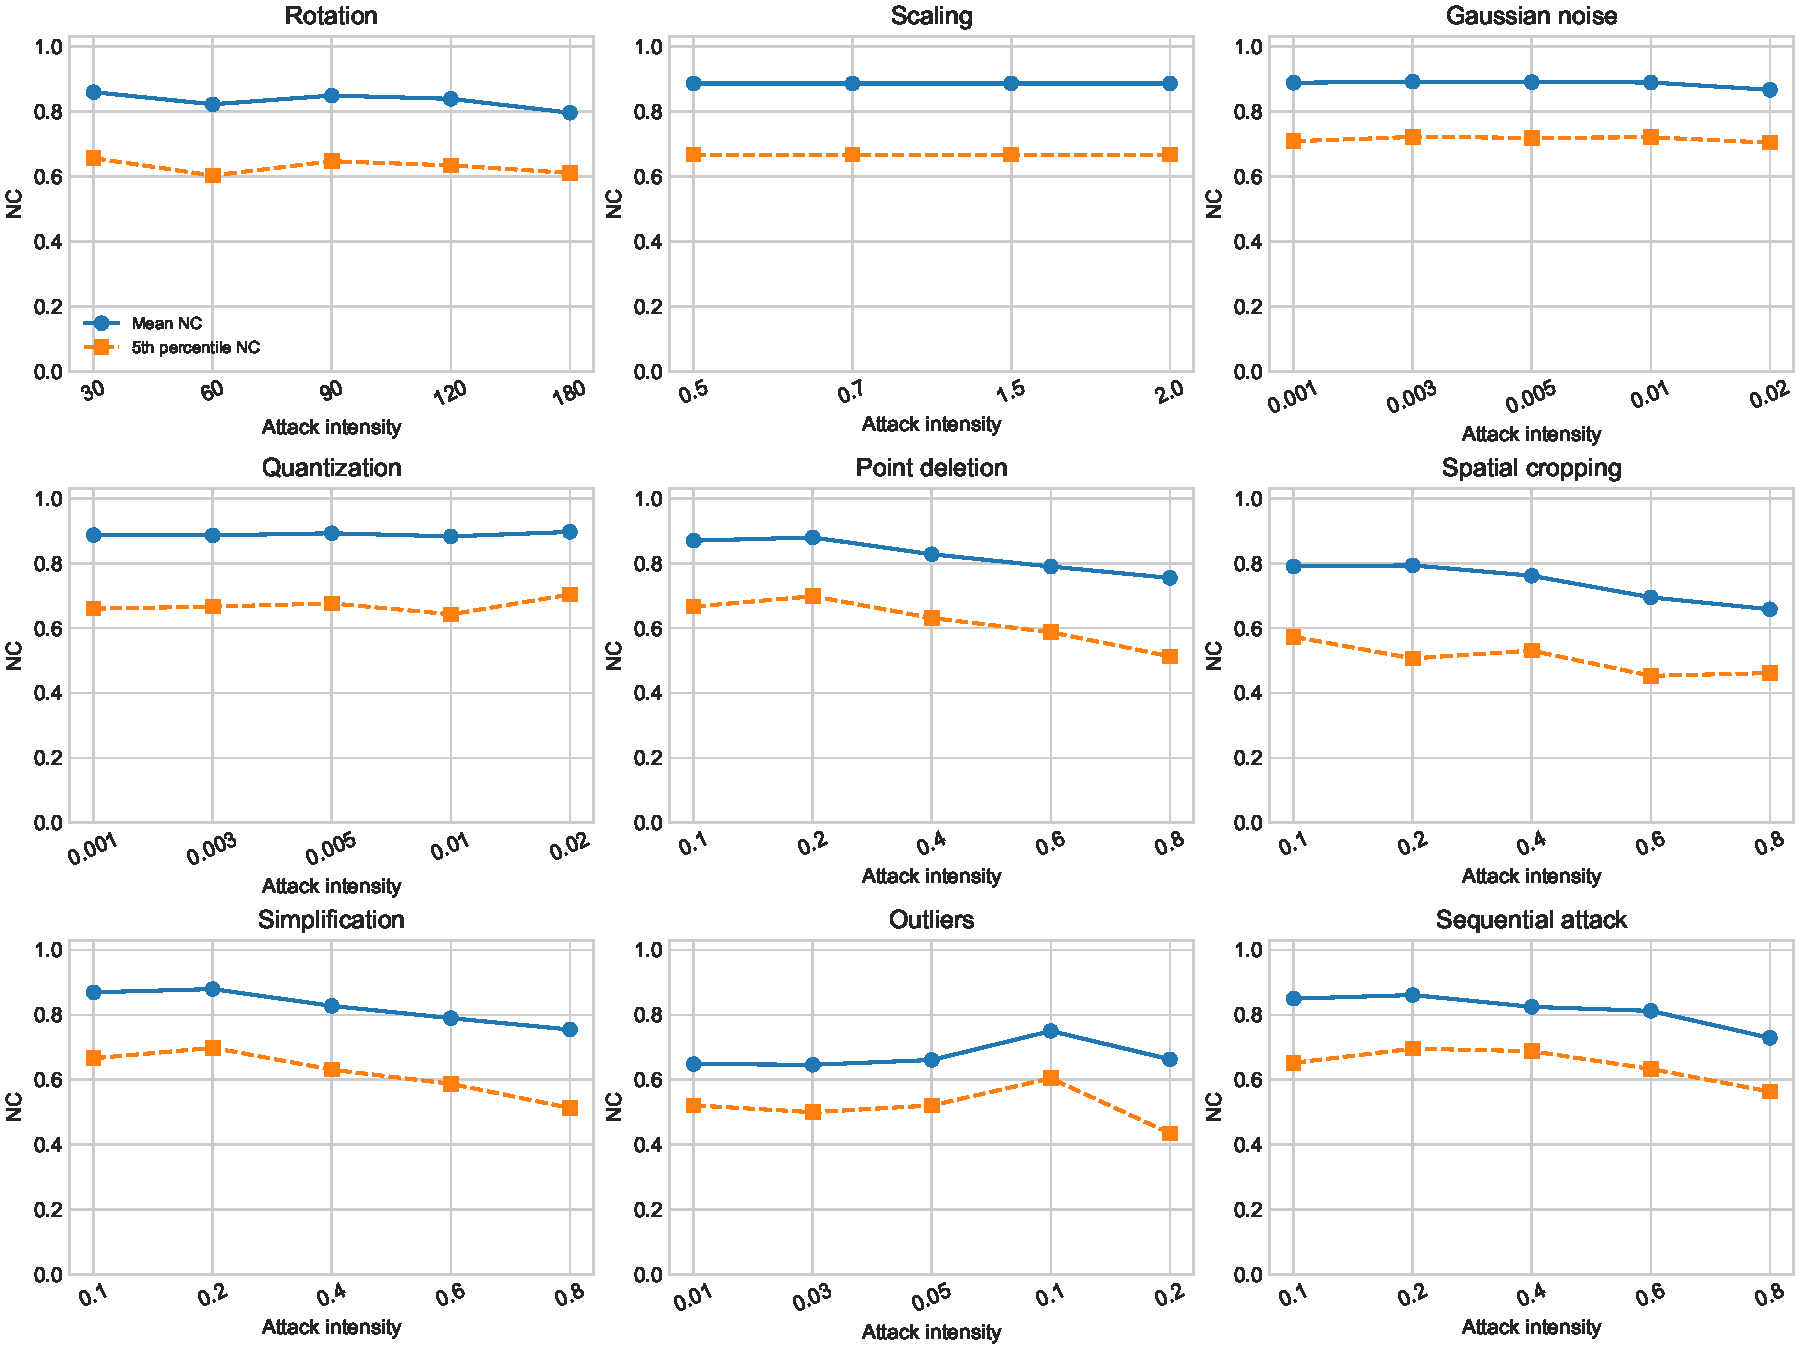
\includegraphics[width=\textwidth]{figures/robustness_grid.pdf}\caption{地域隔离测试集九类攻击的强度--NC曲线。实线为平均NC，虚线为$q_{0.05}$。}\label{fig:robust}\end{figure}
旋转、尺度、噪声和量化全部强度AUC均为1.000。80\%删点与近似简化下平均NC为0.755、AUC为0.957；80\%连续组合攻击下平均NC为0.729、AUC仍为1.000。60\%和80\%裁剪的平均NC分别为0.695和0.658，对应AUC为0.885和0.897。20\%离群点的AUC为\WorstAUC，是全部设置的最差点，说明异常点仍会干扰PCA主轴和局部表示。

\subsection{唯一性与基线比较}
登记指纹异源NC均值为\UniqueMean，q95为\UniqueQ，最大值为\UniqueMax，接近独立平衡二值码的0.5。
\begin{table}[H]\centering\caption{相同地域隔离测试集和攻击实现下的基线比较。}\label{tab:baseline}\begin{tabular}{lcc}\toprule 方法 & 异源NC q95 & 最差AUC \\ \midrule
RadialHist & 0.846 & 0.277 \\
SphericalHist & 0.905 & 0.544 \\
MomentFusion & 0.967 & 0.014 \\
HKReal3DMark & 0.507 & 0.876 \\
\bottomrule\end{tabular}\end{table}
人工基线异源q95达到0.846--0.967，相似城市瓦片容易产生近似统计指纹。MomentFusion虽然特征更多，但同源和异源分布同时集中。\method 将异源q95降至\UniqueQ，并将全攻击强度最差AUC提高到\WorstAUC，支持联合学习稳定性与身份间隔。

\subsection{同载体倾斜摄影方法比较}
\begin{figure}[H]\centering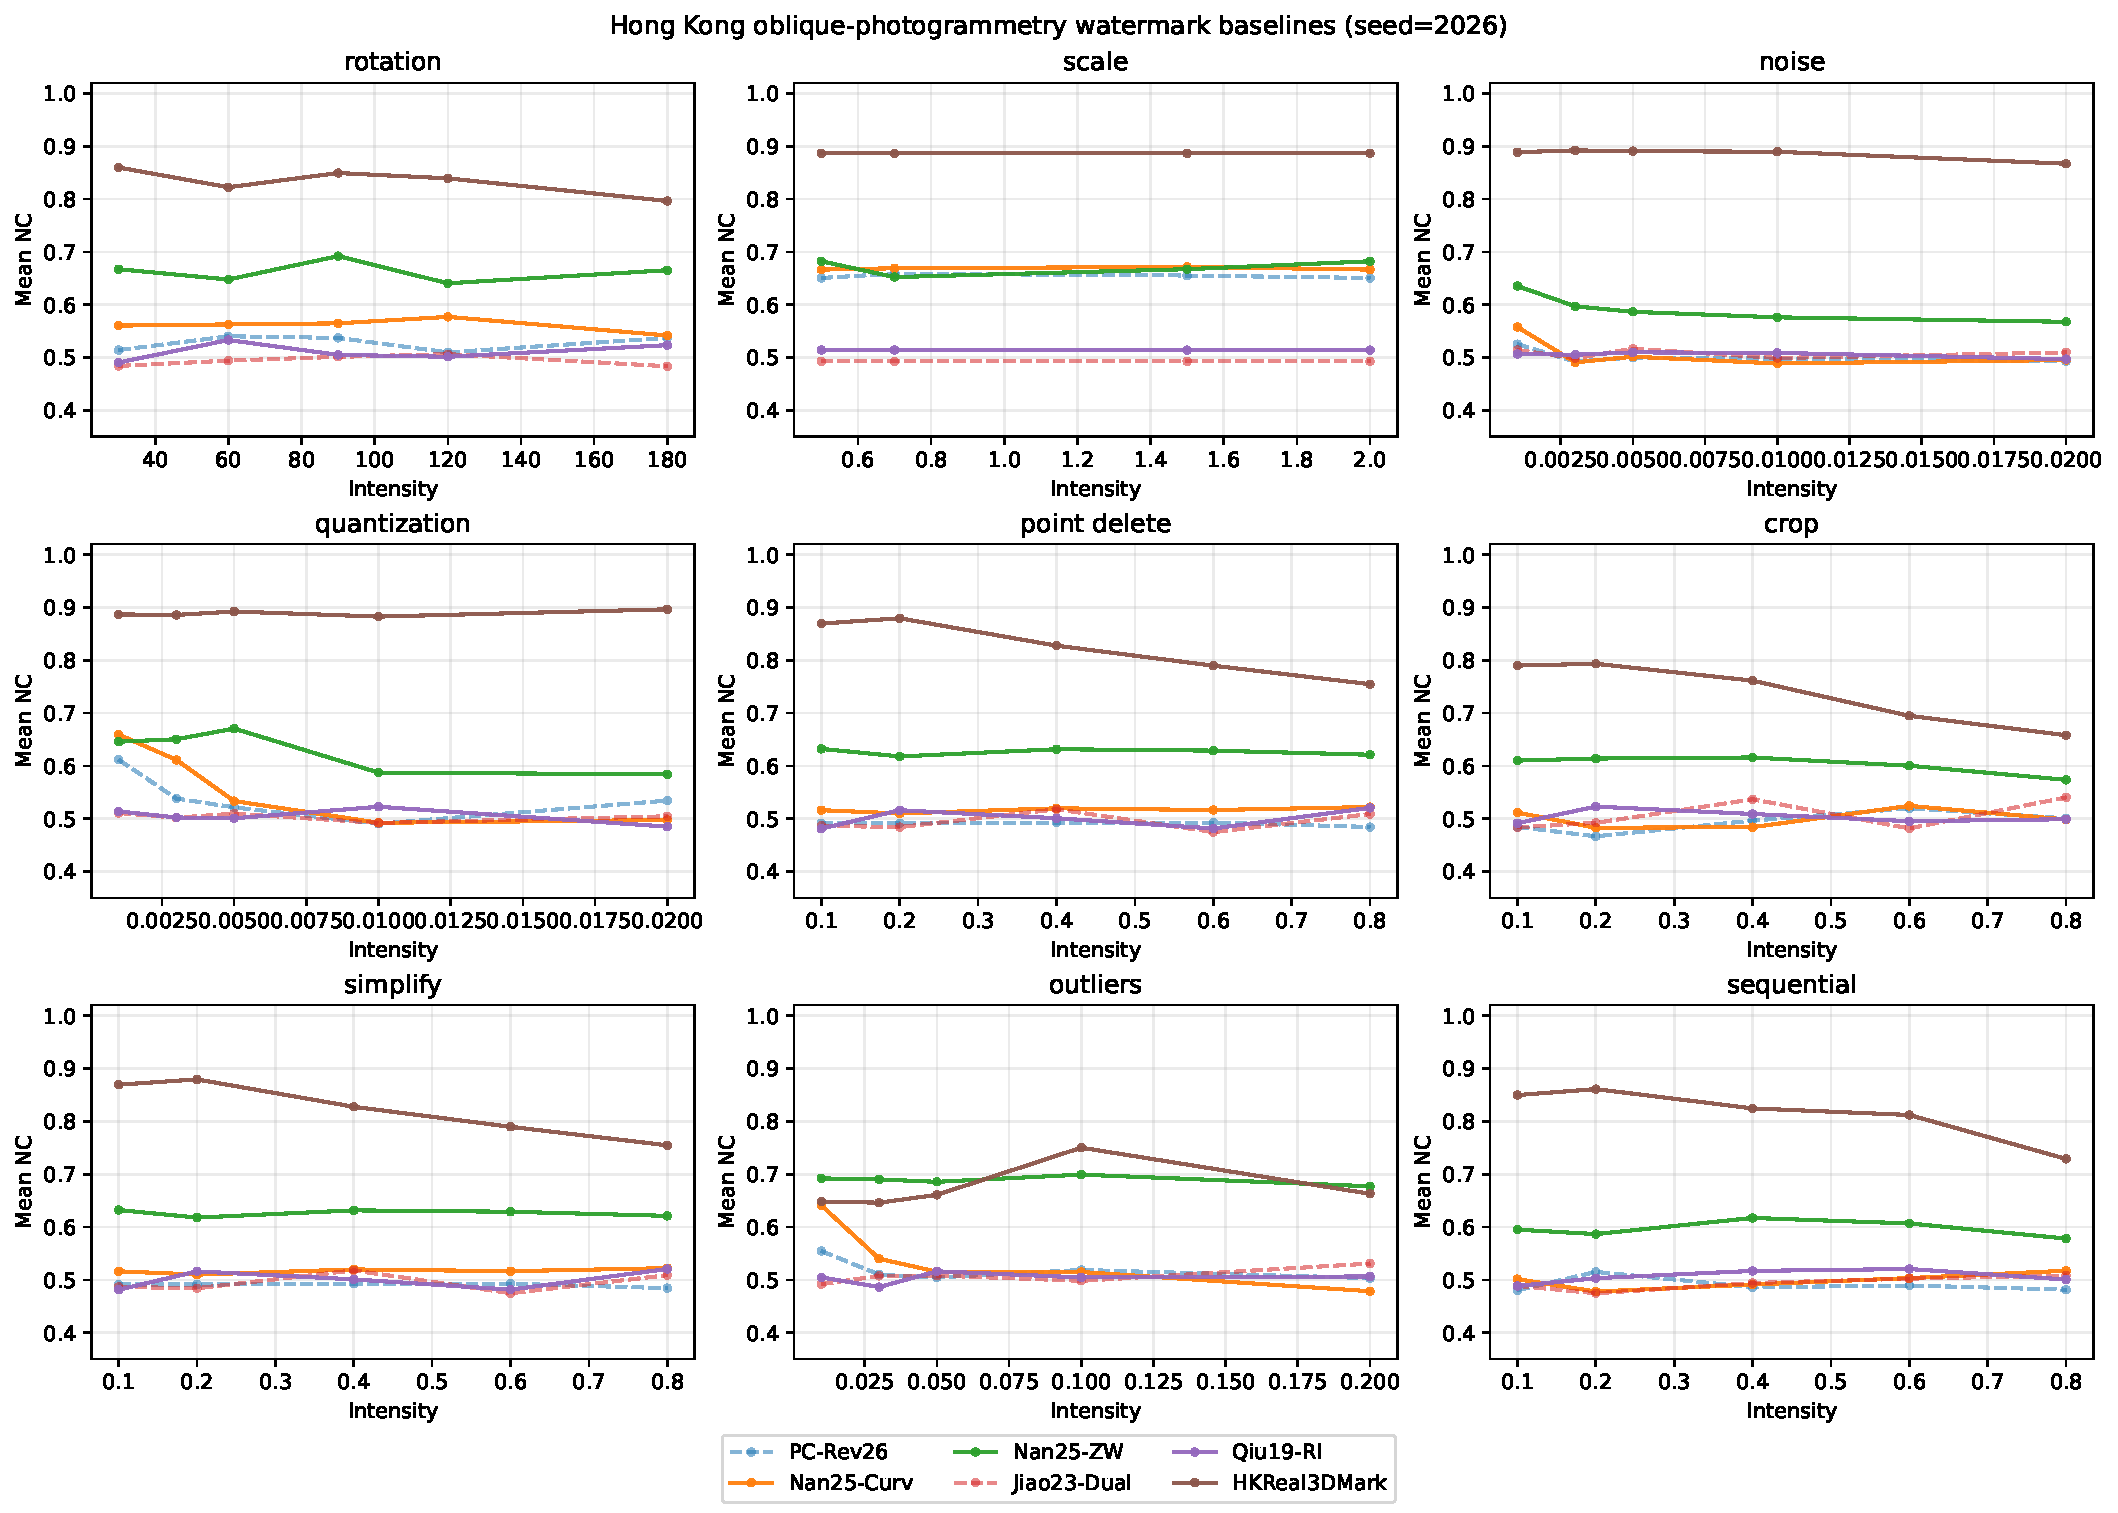
\includegraphics[width=\textwidth]{figures/oblique_baseline_robustness.pdf}\caption{五种倾斜摄影实景三维水印适配方法与本文方法在相同香港测试集上的攻击强度--平均NC曲线。虚线方法未通过无攻击自检。}\label{fig:oblique-baseline}\end{figure}
\begin{table}[H]\centering\caption{同载体方法的无攻击自检、有效位覆盖率及全攻击最差平均NC。星号表示自检失败。}\label{tab:oblique-baseline}\begin{tabular}{lcccc}\toprule
Method & Type & Clean NC & Coverage & Worst NC \\\midrule
PC-Rev26* & Embedded & 0.880 & 0.675 & 0.467 \\
Nan25-Curv & Embedded & 0.951 & 0.704 & 0.478 \\
Nan25-ZW & Zero & 1.000 & 1.000 & 0.568 \\
Jiao23-Dual* & Embedded & 0.823 & 0.874 & 0.475 \\
Qiu19-RI & Embedded & 1.000 & 0.874 & 0.481 \\
HKReal3DMark & Zero & 1.000 & 1.000 & 0.646 \\
\bottomrule\end{tabular}
% * adapted implementation failed the clean self-check\end{table}
PC-Rev26和Jiao23-Dual的无攻击NC分别仅为0.880和0.823，说明论文示例依赖的特征点重分组或纹理分支不能稳定迁移到任意香港瓦片；因此其攻击曲线仅作为适配失败诊断。通过自检的Nan25-Curv、Nan25-ZW和Qiu19-RI的最差平均NC分别为0.478、0.568和0.481，低于本文的0.646。更重要的是，Nan25-ZW在276对异源模型上的NC均值、q95和最大值分别为0.611、0.750和0.844，而本文对应值为\UniqueMean、\UniqueQ 和\UniqueMax，表明偏度统计在相似城市瓦片间存在明显碰撞。

\subsection{轻量性与鲁棒性--唯一性关系}
编码器仅有\ModelParams 个参数，FP32权重约1.1~MB；1024$\times$256投影约1.0~MB。120模型、1800轮的正式训练在RTX~4090上约157秒，峰值显存约1.3~GB。若编码器对所有模型输出同一码字，任意攻击NC都等于1，但认证失效。AUC把异源登记对作为负样本，因而比单独NC更能反映版权认证能力。

\section{讨论}
\subsection{为什么不能直接沿用CityGML语义图模型}
CityGML保存建筑对象、边界面和层级关系，适合对象节点图；香港tile-based B3DM是摄影测量网格，主要信息是三角形几何和纹理。如果将每个三角形强行视为语义节点，不仅图规模巨大，也会虚构不存在的CIM语义。因此本文冻结原CityGML版本作为未来结构化CIM扩展，当前方法改用点集合表示，论文题目和贡献均限定于实景三维。

\subsection{极端攻击与局限性}
80\%单侧裁剪后只剩原模型五分之一，剩余内容可能已不足以代表完整作品。继续追求NC接近1会迫使模型忽略局部差异并损害唯一性。本文仍报告到80\%以展示压力边界，但把20--40\%视为更常见工作区间。

当前研究仍有局限：120个模型来自同一城市，尚不能代表跨城市、跨传感器泛化；点集“简化”是网格降面的近似，后续需加入QEM、重三角化和B3DM--OBJ--GLB往返；个性化登记由干净测试对象在线生成增强视图，属于transductive enrollment，不能外推为未知对象开放集识别；按用户当前实验约束固定一个种子，未估计初始化方差。

\section{结论}
本文提出面向香港Cesium/B3DM实景三维网格的轻量零水印框架\method。方法通过稳健坐标规范化、局部--全局融合编码、多攻击视图学习和仅投影个性化，在不修改源模型的前提下生成1024-bit版权指纹。地域隔离实验表明，模型在刚体变换、噪声、量化、强删点和连续组合攻击下保持较好认证可分性，同时异源NC接近随机平衡码。空间裁剪和高比例离群点仍是主要难点。三维零水印评价不能只展示攻击后NC，必须同时报告异源唯一性和正负分布可分性。
\bibliographystyle{unsrtnat}\bibliography{references}
\end{document}
